\chapter{物理层}\label{CN02}

\section{数据、信号与码元速率}\label{CN02-signal}

数据承载信息，信号是数据在介质中的表示。数字或模拟数据均可通过相应变换形成数字或模拟信号。信源产生数据，信宿接收数据；编码器/解码器处理编码，调制器/解调器处理载波映射。

码元是在固定时间间隔内选择的一种波形或状态。有 \(M\) 种可区分状态，理想等长二进制编码每码元携带 \(\log_2M\) bit：

\[R_b=R_s\log_2M.\]

\(R_s\) 用 Baud（码元/s），\(R_b\) 用 bit/s；每秒已给的码元数直接代入。频率带宽 \(B\) 为频率上下限之差，用Hz；链路数据率意义的带宽用bit/s。

单工只单向；半双工双向交替；全双工双向同时。一条物理线路可按频率、时间或编码承载多个逻辑信道。基带传输直接传基带信号，频带传输通过调制搬移到载波频带。

\section{奈奎斯特极限与香农容量}\label{CN02-capacity}

\par\smallskip
{\fontsize{9.3}{12}\selectfont\setlength{\tabcolsep}{2.5pt}\setlength{\LTleft}{0pt}\setlength{\LTright}{0pt}
\begin{longtable}{@{}>{\raggedright\arraybackslash}p{\dimexpr0.31447\linewidth-2\tabcolsep\relax}>{\raggedright\arraybackslash}p{\dimexpr0.28893\linewidth-2\tabcolsep\relax}>{\raggedright\arraybackslash}p{\dimexpr0.39660\linewidth-2\tabcolsep\relax}@{}}
\toprule
已知条件 & 关系 & 前提 \\

\midrule\endfirsthead\toprule
已知条件 & 关系 & 前提 \\

\midrule\endhead\bottomrule\endfoot
无噪声低通信道、带宽 \(B\) & \(R_s\le2B\)；\(R_b\le2B\log_2M\) & 无码间串扰，\(M\)为可区分状态数 \\

带限高斯噪声信道 & \(C=B\log_2(1+S/N)\) & \(S/N\)为无量纲功率比；可靠传输理论极限 \\

信噪比 \(\gamma\) dB & \(S/N=10^{\gamma/10}\) & 30 dB对应1000 \\

\end{longtable}}
\par\smallskip

同时给出固定调制状态数和信噪比时，按教材信道模型分别计算两项上界，取有效限制的较小值。仅提高信噪比，固定状态数仍可能限制速率。采样次数超过 \(2B\) 不能增加带限信道的独立码元数。

\par\medskip\Needspace{4\baselineskip}\noindent\hypertarget{CN02-E01}{}\label{CN02-E01}\textbf{例 2-1}\par\nobreak\smallskip

在一条带宽为200 kHz的无噪声信道上，若采用4个幅值的 ASK 调制，则该信道的最大数据传输速率是（　）。

A. 200 kb/s　B. 400 kb/s　C. 800 kb/s　D. 1600 kb/s

\par\medskip\Needspace{4\baselineskip}\noindent\hypertarget{CN02-E02}{}\label{CN02-E02}\textbf{例 2-2}\par\nobreak\smallskip

某信道带宽为10 MHz，信噪比为30 dB，采用 QAM-32 调制。若带宽提高到20 MHz，信噪比提高到40 dB，则信道的极限数据传输速率大约提高到原来的（　）倍。

A. 2　B. 2.2　C. 2.4　D. 2.6

\section{线路编码与调制}\label{CN02-coding}

\par\smallskip
\begin{wideblock}
{\fontsize{9.3}{12}\selectfont\setlength{\tabcolsep}{2.5pt}\setlength{\LTleft}{0pt}\setlength{\LTright}{0pt}
\begin{longtable}{@{}>{\raggedright\arraybackslash}p{\dimexpr0.23300\linewidth-2\tabcolsep\relax}>{\raggedright\arraybackslash}p{\dimexpr0.36840\linewidth-2\tabcolsep\relax}>{\raggedright\arraybackslash}p{\dimexpr0.39860\linewidth-2\tabcolsep\relax}@{}}
\toprule
编码 & 逐位规则 & 同步与代价 \\

\midrule\endfirsthead\toprule
编码 & 逐位规则 & 同步与代价 \\

\midrule\endhead\bottomrule\endfoot
NRZ不归零 & 每位保持相应电平 & 长串相同位可缺少跳变 \\

RZ归零 & 前半位按数据取电平，后半位回零 & 每位含回零，占更多变化能力 \\

NRZI & 位起点是否跳变表意，位中保持 & 0/1约定按题意；某种长连码可缺少跳变 \\

曼彻斯特 & 每位中点必跳，方向表意 & 中点同步，每位占两个半位区间 \\

差分曼彻斯特 & 中点必跳，起点是否跳变表意 & 首位须给前一电平；依赖相对关系 \\

\end{longtable}}
\end{wideblock}
\par\smallskip

本图约定NRZ低0高1、NRZI起点跳变为0、曼彻斯特中点上跳为0、差分曼彻斯特起点跳变为0，差分初始电平为高。题目约定优先。

\begin{figure}[H]
\centering
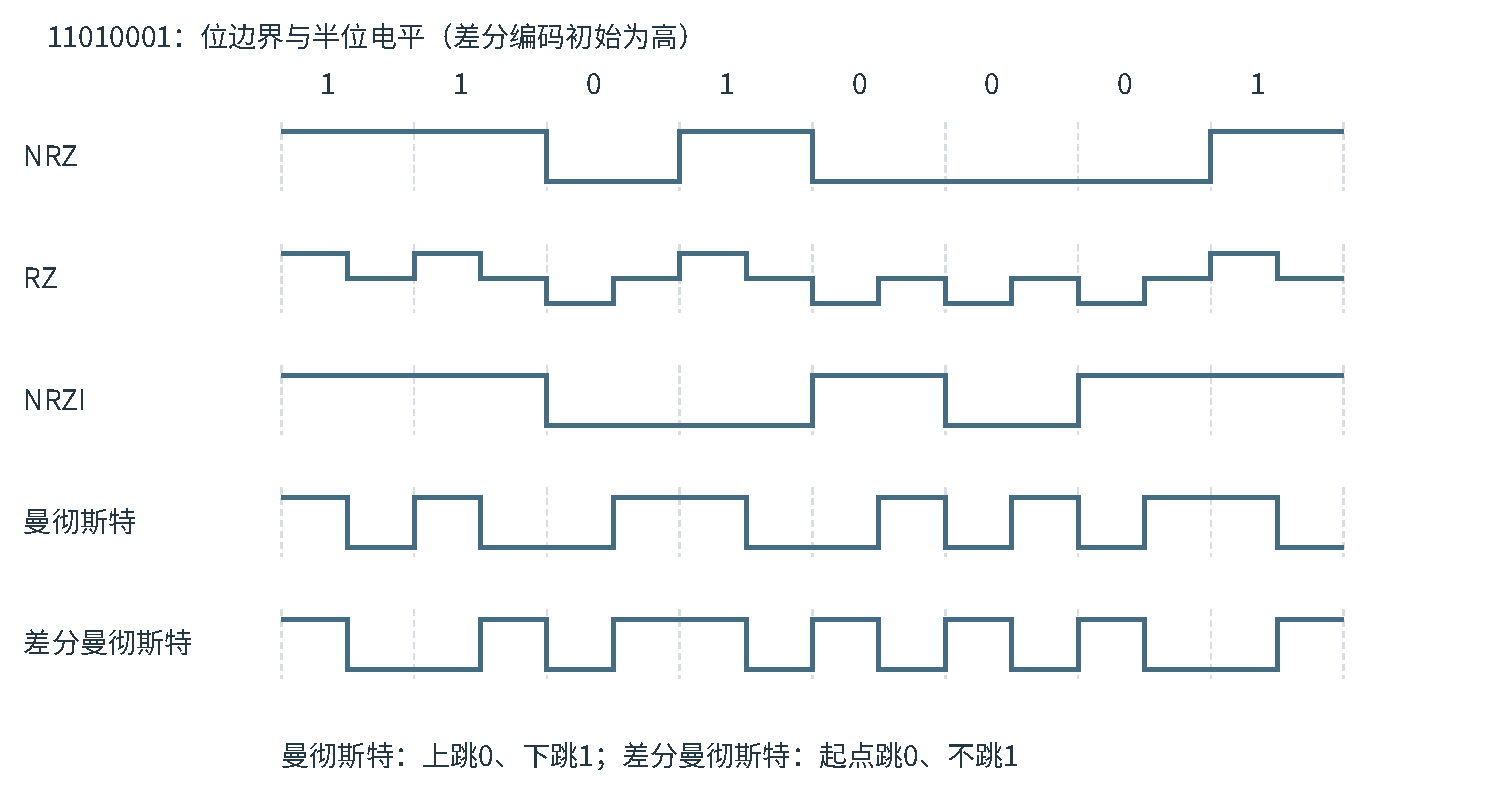
\includegraphics[width=\linewidth,height=108mm,keepaspectratio]{figures/CN_course_five_codes.pdf}
\caption{比特串11010001的五种编码}\label{cn-course-five-codes}
\end{figure}

每秒最多承载 \(2R\) 个半位信号区间时，曼彻斯特比特率至多 \(R\)；若题给最终比特率，直接使用。4B/5B效率为 \(4/5\)，传同量数据需线路比特数乘 \(5/4\)。

ASK改变振幅，FSK改变频率，PSK改变相位，QAM组合振幅与相位。4种振幅\ensuremath{\times}4种相位在波形互不重合时为16态，每码元4 bit；状态数按实际可区分的星座点计算。

\section{PCM采样、量化与编码}\label{CN02-pcm}

PCM流程：采样取得离散时刻幅值，量化到有限级别，编码成比特。理想带限模拟信号最高频率为 \(f_{max}\)：

\[f_s\ge2f_{max},\qquad R_b=f_s q,\]

其中 \(q\) 为每样本编码位数，量化级数最多 \(2^q\)，上式未计额外信道编码。8 kHz采样、每样本8 bit得到64 kb/s。采样定理约束信号恢复，奈氏码元极限约束传输，两者按各自场景使用。

\section{传输介质与物理制式}\label{CN02-media}

\par\smallskip
\begin{wideblock}
{\fontsize{9.3}{12}\selectfont\setlength{\tabcolsep}{2.5pt}\setlength{\LTleft}{0pt}\setlength{\LTright}{0pt}
\begin{longtable}{@{}>{\raggedright\arraybackslash}p{\dimexpr0.35389\linewidth-2\tabcolsep\relax}>{\raggedright\arraybackslash}p{\dimexpr0.64611\linewidth-2\tabcolsep\relax}@{}}
\toprule
介质 & 性质与适用条件 \\

\midrule\endfirsthead\toprule
介质 & 性质与适用条件 \\

\midrule\endhead\bottomrule\endfoot
双绞线 & 绞合减小电磁干扰；屏蔽型再加屏蔽结构 \\

同轴电缆 & 内导体、绝缘层、外导体屏蔽层；速率仍取决于标准、长度和设备 \\

多模光纤 & 多种空间模式，模间色散展宽脉冲，限制距离和速率 \\

单模光纤 & 单一空间模式，减轻模间色散，适合较长距离及高容量；可另做波分复用 \\

无线电、微波、红外 & 传播条件依频率而定；地面微波常要求视距，高轨卫星传播时延大 \\

\end{longtable}}
\end{wideblock}
\par\smallskip

光纤电绝缘、抗电磁干扰、衰减低；容量与传播速度分别计算。频率、波长满足 \(v=f\lambda\)，真空中 \(v=c\)。介质位于物理层之下，物理层规定其信号收发方式。

10BASE5：10 Mb/s、基带、传统粗同轴单段500 m；10BASE2最大段常取185 m；10BASE-T使用双绞线。100BASE-T主要使用双绞线。曼彻斯特适用于传统10 Mb/s以太网，更高速制式按相应物理标准取编码。

\section{物理层接口四类特性}\label{CN02-interface}

\par\smallskip
{\fontsize{9.3}{12}\selectfont\setlength{\tabcolsep}{2.5pt}\setlength{\LTleft}{0pt}\setlength{\LTright}{0pt}
\begin{longtable}{@{}>{\raggedright\arraybackslash}p{\dimexpr0.35679\linewidth-2\tabcolsep\relax}>{\raggedright\arraybackslash}p{\dimexpr0.64321\linewidth-2\tabcolsep\relax}@{}}
\toprule
特性 & 规定内容 \\

\midrule\endfirsthead\toprule
特性 & 规定内容 \\

\midrule\endhead\bottomrule\endfoot
机械 & 连接器形状、尺寸、接点排列 \\

电气 & 电压、电平、阻抗、传输速率 \\

功能 & 各信号线承担的作用 \\

规程 & 信号出现与双方动作的顺序 \\

\end{longtable}}
\par\smallskip

\par\medskip\Needspace{4\baselineskip}\noindent\hypertarget{CN02-E03}{}\label{CN02-E03}\textbf{例 2-3}\par\nobreak\smallskip

下列选项中，不属于物理层接口规范定义范畴的是（　）。

A. 接口形状　B. 引脚功能　C. 物理地址　D. 信号电平

\section{中继器与集线器}\label{CN02-repeater}

中继器判决、整形并再生比特信号；已判错的比特无法靠再生恢复。它不检查MAC、不学习转发表。连接不同介质须满足速率、编码及协议等兼容条件。

集线器是多端口中继器，一个端口收到比特便向其他端口转送，所有站共享带宽和冲突域。\(n\)站共享 \(R\) 的理想均分为 \(R/n\)，实际竞争和协议开销另计。

最远站传播时延先累计途经各段距离，再除传播速度；冲突反馈需要往返，设备时延也计入。传统10BASE5的5-4-3规则：最多5段、4个中继设备，其中3段可挂接终端；其他标准按各自距离、延迟和连接规范。
